% ============================================================
% 第二章 相关技术
% ============================================================

\section{相关技术}

\subsection{图片插入示例}

图~\ref{fig:neural-network}展示了一个深度神经网络结构示例。

% 单图示例
\begin{figure}[htbp]
    \centering
    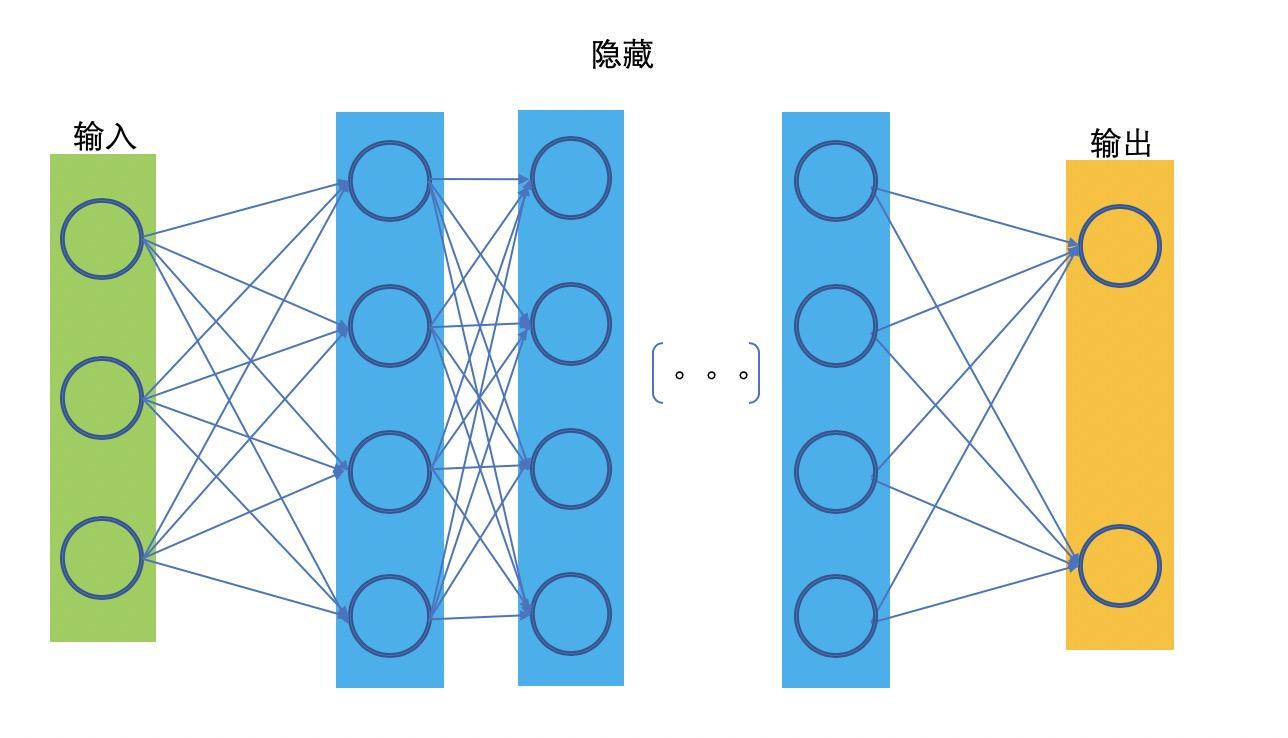
\includegraphics[width=0.8\textwidth]{figture/example}
    \caption{深度神经网络结构示意图}
    \label{fig:neural-network}
\end{figure}

\subsection{公式排版示例}

行内公式示例：$E = mc^2$，$\alpha + \beta = \gamma$。

独立编号公式示例：
\begin{equation}
    \int_{a}^{b} f(x) \, dx = F(b) - F(a)
    \label{eq:integral}
\end{equation}

多行对齐公式示例：
\begin{align}
    \nabla \cdot \vec{E} &= \frac{\rho}{\varepsilon_0} \label{eq:maxwell1} \\
    \nabla \times \vec{E} &= -\frac{\partial \vec{B}}{\partial t} \label{eq:maxwell2}
\end{align}

公式~\eqref{eq:integral}展示了微积分基本定理，公式~\eqref{eq:maxwell1}和\eqref{eq:maxwell2}是麦克斯韦方程组的一部分。

\subsection{表格排版示例}

表~\ref{tab:three-line}展示了标准三线表的排版效果。

% 三线表示例
\begin{table}[htbp]
    \centering
    \caption{实验结果对比表}
    \label{tab:three-line}
    \begin{tabular}{ccc}
        \toprule
        \textbf{方法} & \textbf{准确率(\%)} & \textbf{运行时间(s)} \\
        \midrule
        方法A & 92.5 & 1.23 \\
        方法B & 94.8 & 1.56 \\
        方法C & 96.2 & 2.01 \\
        \bottomrule
    \end{tabular}
\end{table}

\subsection{本章小结}

本章展示了LaTeX模板的核心功能：图片插入、数学公式排版（行内公式、独立公式、多行对齐公式）、三线表排版等功能。
